\chapter{Численная схема решения на основе метода конечных элементов}\label{ch:NumericalMethods}

\section{Общие сведения о методе конечных элементов}\label{sec:NumericalMethods/GeneralAboutFEM}

В качестве численного метода решения для уравнений (\ref{eq:StationaryHeatEquation}) и (\ref{eq:EquilibriumEquation}) выбрем метод конечных элементов с использованием изопараметрических конечных элементов \cite{Zienkiewicz, Bathe}. Для этого на области $S$ введём сетку конечно-элементной модели $S_h$, которая включает в себя множества номеров узлов и связей между ними, образующих непосредственно сами элементы. Каждый элемент $e \in S_h$ содержит в себе множества узлов $\{ x_i \}_{i \in I^{e}}$ и базисных функций $\{ N_i^{e} \}_{i \in I^{e}}$ таких, что
\begin{gather*}
	N_i^{e}(\boldsymbol{x}_j) = \delta_{ij}, \quad i,j \in I^{e}, \\
	N_i^{e} (\boldsymbol{x}) = 0, \quad \boldsymbol{x} \notin S^{e}, \\
	\sum\limits_{i \in I^{e}} N_i^{e}(\boldsymbol{x}) = 1, \quad \boldsymbol{x} \in S^{e},
\end{gather*}
где $I^{e}$ --- множество индексов узлов элемента $e$;
$\delta_{ij}$ --- дельта Кронекера;
$\boldsymbol{x}_j$~---~значения глобальных координат в узлах сетки;
$S^{e}$ --- область \mbox{элемента $e$.}

Для каждого конечного элемента $e$ введём локальную систему координат $O \xi_{1}^{e} \xi_{2}^{e}$. Отображение из локальной системы координат $O \xi_{1}^{e} \xi_{2}^{e}$ в глобальную $O \text{x}_1 \text{x}_2$ будем строить следующим образом
\begin{gather*}
	\boldsymbol{x}(\boldsymbol{\xi}^{e}) = N_i^{e} \left( \boldsymbol{\xi}^{e} \right) \boldsymbol{x}_i,
	\quad
	i \in I^{e}, \ e \in S_h.
\end{gather*}
Тогда матрицу Якоби перехода из локальной системы координат в глобальную можем представить в виде
\begin{gather*}
	\widehat{\text{\textbf{J}}}^{e} =
	\left( \dfrac{\partial \boldsymbol{\xi}^{e}}{\partial \boldsymbol{x}} \right) =
	\left( \dfrac{\partial \boldsymbol{x}}{\partial \boldsymbol{\xi}^{e}} \right)^{-1} \approx
	\left( \boldsymbol{x}_i \dfrac{\partial N_i^{e}}{\partial \boldsymbol{\xi}^{e}} \right)^{-1},
\end{gather*}
а вычисление производных функций форм относительно глобальных координат примет следующий вид
\begin{gather*}
	\dfrac{\partial N_i^{e}}{\partial x_k} =
	\dfrac{\partial N_i^{e}}{\partial \xi_j^{e}}
	\dfrac{\partial \xi_j^{e}}{\partial x_k}.
\end{gather*}

Аппроксимированную границу $\Gamma_h \subset S_h$ представим в виде набора одномерных элементов, располагающихся на гранях двумерных элементов. При интегрировании внешних воздействий на границах области также возникает необходимость в аппроксимации якобиана, формулу которого можно определить в следующем виде
\begin{gather*}
	J^{e} = \sqrt{
		\sum\limits_{j=1}^{2} 
		\left( 
			x_{ji} \dfrac{\partial N_i^{e}}{\partial \xi^{e}}
		\right)^2
	},
	\quad
	i \in I^{e}, \
	e \in \Gamma_h.
\end{gather*}

\section{Аппроксимация уравнений}\label{sec:NumericalMethods/EquationApproximation}

Спроецируем уравнения (\ref{eq:StationaryHeatEquation}) и (\ref{eq:EquilibriumEquation}) на функцию $N_n^{e}$, где $n \in I^{e}, e \in S_h$
\begin{gather*}
	\int\limits_S N_n^{e} \left( \nabla \cdot \boldsymbol{q} - q_V \right) dS = 0,
	\\
	\int\limits_S N_n^{e} (\nabla \cdot \widehat{\boldsymbol{\sigma}} - \boldsymbol{b}) dS = \boldsymbol{0}.
\end{gather*}
Проинтегрируем по частям первое слагаемое каждого уравнения, тогда пользуясь формулой Грина получаем следующие равенства
\begin{gather*}
	\int\limits_S \nabla N_n^{e} \cdot \boldsymbol{q} dS -
	\int\limits_{\partial S} \boldsymbol{n} \cdot \boldsymbol{q} d\Gamma =
	\int\limits_S N_n^{e} q_V dS, \\
	\int\limits_S \nabla N_n^{e} \cdot \widehat{\boldsymbol{\sigma}} dS -
	\int\limits_{\partial S} \boldsymbol{n} \cdot \widehat{\boldsymbol{\sigma}} d\Gamma =
	\int\limits_S N_n^{e} \boldsymbol{b} dS.
\end{gather*}
Подставим определения граничных условий уравнения теплопроводности (\ref{eq:ThermalBoundaries}) и уравнения равновесия (\ref{eq:StressBoundaries}), интегралы по границе $\partial S$ разбиваем на суммы интегралов
\begin{gather*}
	\int\limits_S \nabla N_n^{e} \cdot \boldsymbol{q} dS +
	\int\limits_{\Gamma_3} \alpha N_n^{e} T d\Gamma =
	\int\limits_S N_n^{e} q_V dS +
	\int\limits_{\Gamma_2} N_n^{e} f d\Gamma +
	\int\limits_{\Gamma_3} \alpha N_n^{e} T_a d\Gamma, \\
	\int\limits_S \nabla N_n^{e} \cdot \widehat{\boldsymbol{\sigma}} dS =	
	\int\limits_S N_n^{e} \boldsymbol{b} dS +
	\int\limits_{\Gamma_5} N_n^{e} \boldsymbol{p} d\Gamma.
\end{gather*}
Теперь воспользуемся определениями плотности теплового потока (\ref{eq:BiotFourier}) и тензора напряжений (\ref{eq:DuamelNeumann}), а также определением оператора (\ref{eq:IntegroDiffOperator}) и в итоге приходим к следующим равенствам относящимся к уравнению теплопроводности
\begin{multline}
	\label{eq:ThermalIntegrate}
	\int\limits_S \nabla N_n^{e} \cdot 
	\left(
		-p_1 \widehat{\boldsymbol{\lambda}} \cdot \nabla T dS
		-
		p_2 	\int\limits_{S'(\boldsymbol{x}) \cap S} 
	\varphi(\boldsymbol{x}, \boldsymbol{x}') \widehat{\boldsymbol{\lambda}} \cdot \nabla T
	dS'(\boldsymbol{x})
	\right) dS 
	+ \\ +
	\int\limits_{\Gamma_3} \alpha N_n^{e} T d\Gamma 
	=
	\int\limits_S N_n^{e} q_V dS +
	\int\limits_{\Gamma_2} N_n^{e} f d\Gamma + 
	\int\limits_{\Gamma_3} \alpha N_n^{e} T_a d\Gamma,
\end{multline}
и уравнению равновесия
\begin{multline}
	\label{eq:StressIntegrate}
	\int\limits_S \nabla N_n^{e} \cdot 
	\Bigg( 	
		p_1 \widehat{\text{\textbf{C}}} \cdot \cdot \left( \widehat{\boldsymbol{\varepsilon}} - \widehat{\boldsymbol{\alpha}}^T \Delta T \right) dS
	+ \\ +
	p_2 \int\limits_{S'(\boldsymbol{x}) \cap S} 
	\varphi(\boldsymbol{x}, \boldsymbol{x}') 
	\widehat{\text{\textbf{C}}} \cdot \cdot \left( \widehat{\boldsymbol{\varepsilon}} - \widehat{\boldsymbol{\alpha}}^T \Delta T \right) dS'(\boldsymbol{x})
	\Bigg) dS
	= \\ =
	\int\limits_S N_n^{e} \boldsymbol{b} dS +
	\int\limits_{\Gamma_5} N_n^{e} \boldsymbol{p} d\Gamma.
\end{multline}

Аппроксимируем температуру $T$ и вектор перемещения $\boldsymbol{u}$ на элементе
\begin{gather*}
	T (\boldsymbol{x}) = T_m N_m^e (\boldsymbol{x}),
	\quad
	\boldsymbol{u} (\boldsymbol{x}) = \boldsymbol{u}_m N_m^e (\boldsymbol{x}),
	\quad
	\boldsymbol{x} \in S^e,
\end{gather*}
где $T_m$ и $\boldsymbol{u}_m$ --- искомые значения температуры и вектора перемещения в узле $m \in I^e$. Тогда аппроксимация градиента температуры и тензора деформации $\widehat{\boldsymbol{\varepsilon}}$ примут следующий вид
\begin{gather}
	\label{eq:ApproxTemperatureGradient}
	\nabla T = T_m N^e_{m,k} \boldsymbol{e}_k,
	\\
	\label{eq:ApproxStrain}
	\widehat{\boldsymbol{\varepsilon}} = 
	\dfrac{1}{2} \left( \boldsymbol{u}_m \nabla N_m^e + (\boldsymbol{u}_m \nabla N_m^e)^T \right) =
	\dfrac{1}{2} ( u_{mk} N_{m,l}^e + u_{ml} N_{m,k}^e) \boldsymbol{e}_k \otimes \boldsymbol{e}_l.
\end{gather}
Теперь подставим аппроксимированные значения в уравнения (\ref{eq:ThermalIntegrate}) и (\ref{eq:StressIntegrate}) и перейдя к индексной форме записи, а также разделив локальные и нелокальные слагаемые, получим системы уравнений для уравнения теплопроводности
\begin{multline}
	\label{eq:ThermalIntegrateIndices}
	-p_1 T_m
	\int\limits_S
	\lambda_{ij} N_{n, i}^{e} N_{m, j}^{e} dS
	-
	p_2 T_{m'}
	\int\limits_S
	N_{n, i}^{e}
	\int\limits_{S'(\boldsymbol{x}') \cap S}
	\varphi( \boldsymbol{x}, \boldsymbol{x}' )
	\lambda_{ij}
	N_{m', j}^{e'} dS'(\boldsymbol{x}) dS
	+\\+
	T_m \int\limits_{\Gamma_3} \alpha N_n^{e} N_m^{e} d\Gamma
	=
	\int\limits_S N_n^{e} q_V dS +
	\int\limits_{\Gamma_2} N_n^{e} f d\Gamma +
	\int\limits_{\Gamma_3} \alpha N_n^{e} T_a(\boldsymbol{x}) d\Gamma,
\end{multline}
и уравнения равновесия
\begin{multline}
	\label{eq:StressIntegrateIndices}
	p_1 \int\limits_S N_{n,i}^{e} C_{ijkl} \varepsilon_{kl} dS
	+
	p_2 \int\limits_S N_{n, i}^{e} \int\limits_{S'(\boldsymbol{x}) \cap S}
	\varphi(\boldsymbol{x}, \boldsymbol{x}') C_{ijkl} \varepsilon_{kl} dS'(\boldsymbol{x}) dS
	= \\ =
	p_1 \int\limits_S N_{n,i}^{e} C_{ijkl} \alpha_{kl} \Delta T dS +
	p_2 \int\limits_S N_{n,i}^{e}
	\int\limits_{S'(\boldsymbol{x}) \cap S} 
	\varphi(\boldsymbol{x}, \boldsymbol{x}')
	C_{ijkl} \alpha_{kl} \Delta T dS'(\boldsymbol{x}) dS 
	+ \\ +
	\int\limits_S N_n^{e} b_j dS +
	\int\limits_{\Gamma_5} N_n^{e} p_j d\Gamma,
\end{multline}
где $i,j,k,l = \overline{1, 2}$; $m, n \in I^e$; $m, n \in I^e$; $m' \in I^{e'}$; $e \in S_h$; $e' \in S'_h$; $S'_h$ --- аппроксимированная зона нелокального влияния, детали аппроксимации которой рассмотрим далее в следующей главе.

После интегрирования, о котором пойдёт речь в следующем разделе, итоговые системы можно записать в матрично-векторном виде
\begin{gather}
	\label{eq:ThermalSLAE}
	\left( p_1 \widehat{\textbf{K}}^L_T + p_2 \widehat{\textbf{K}}^{NL}_T + \widehat{\textbf{K}}^{\alpha}_T \right) \cdot \textbf{T} = \textbf{Q} + \textbf{F} + \textbf{T}^{\alpha}, \\
	\label{eq:StressSLAE}
	\left( p_1 \widehat{\textbf{K}}^L_E + p_2 \widehat{\textbf{K}}^{NL}_E \right) \cdot \widehat{\textbf{U}} = p_1 \widehat{\textbf{E}}^L + p_2 \widehat{\textbf{E}}^{NL} + \widehat{\textbf{B}} + \widehat{\textbf{P}}.
\end{gather}
где $\widehat{\textbf{K}}^L_T$ и $\widehat{\textbf{K}}^{NL}_T$~---~матрицы локальной и нелокальной теплопроводности;
$\widehat{\textbf{K}}^{\alpha}_T$~---~матрица теплопередачи;
$\textbf{T}$ --- вектор искомых узловых значений температуры;
$\textbf{Q}$ и $\textbf{F}$ --- векторы дискретизированных внутренних и внешних источников и стоков теплоты;
$\textbf{T}^{\alpha}$ --- вектор дискретизированной теплопередачи;
$\widehat{\textbf{K}}^L_E$ и $\widehat{\textbf{K}}^{NL}_E$ --- матрицы локальной и нелокальной жёсткости;
$\widehat{\textbf{U}}$~---~вектор искомых узловых перемещений;
$\widehat{\textbf{B}}$ и $\widehat{\textbf{P}}$ --- векторы дискретизированных плотностей объёмных и поверхностных сил;
$\widehat{\textbf{E}}^L$ и $\widehat{\textbf{E}}^{NL}$ --- векторы локального и нелокального температурного линейного расширения.
В силу того, что матрицы $\widehat{\textbf{K}}^L_E$ и $\widehat{\textbf{K}}^{NL}_E$ имеют блочную структуру, с размером блока $2 \times 2$, для удобства дальнейшего изложения будем представлять их в виде аналогов (по количеству индексов) тензоров четвёртого ранга, где первые два индекса обозначают строку и столбец с указанием блока, а вторые --- строку и столбец внутри блока.
Аналогично представим векторы \mbox{$\widehat{\textbf{U}}$, $\widehat{\textbf{B}}$, $\widehat{\textbf{P}}$, $\widehat{\textbf{E}}^L$ и $\widehat{\textbf{E}}^{NL}$} в виде тензоров второго ранга, где первый индекс соответствует номеру узла, а второй --- номеру координатной компоненты.

\section{Ассемблирование систем уравнений}\label{sec:NumericalMethods/SLAEAssembling}

Рассмотрим более подробно вопрос ассемблирования систем уравнений (\ref{eq:ThermalSLAE}) и (\ref{eq:StressSLAE}), которые получаем после интегрирования систем (\ref{eq:ThermalIntegrateIndices}) и (\ref{eq:StressIntegrateIndices}). Для удобства расмотрим  каждое из слагаемых поотдельности. Но прежде чем это сделать нам потребуется ввести определения блоков матрицы теплопроводности $\widetilde{\textbf{K}}_{nm}^{e_1 e_2}$ и жёсткости $\widehat{\textbf{K}}_{nm}^{e_1 e_2}$, стоящих в $n$-ой строке и $m$-ом столбце соответствующих матриц
\begin{gather}
	\label{eq:ThermalBlock}
	\widetilde{\textbf{K}}_{nm}^{e_1 e_2} (\boldsymbol{x}, \boldsymbol{y}) =
	\lambda_{ij} N_{n,i}^{e_1} (\boldsymbol{x}) N_{n,j}^{e_1} (\boldsymbol{y})
	\boldsymbol{E}_n \otimes \boldsymbol{E}_m, \\
	\label{eq:StressBlock}
	\widehat{\textbf{K}}_{nm}^{e_1 e_2} (\boldsymbol{x}, \boldsymbol{y}) = 
	C_{ijkl} N_{n,k}^{e_1} (\boldsymbol{x}) N_{m,l}^{e_2} (\boldsymbol{y}) \boldsymbol{e}_i \otimes \boldsymbol{e}_j \otimes \boldsymbol{E}_n \otimes \boldsymbol{E}_m,
\end{gather}
где $i,j,k,l = \overline{1,2}$; $n,m = \overline{1,L}$; $\boldsymbol{E}_n$ --- единичный вектор размерности $M$; $M$ --- количество узлов в сетке $S_h$. Далее, для общности записи будем использовать блок $\textbf{K}_{nm}^{e_1 e_2}$, который будет играть роль блока матрицы теплопроводности или жёсткости в зависимости от контекста.

Рассмотрим матричные слагаемые с множителем $p_1$, которые достаточно легко аппроксимируем классической конечно-элементной процедурой \cite{Zienkiewicz, Bathe}. После её применения ассамблированную матрицу можно записать следующим образом
\begin{gather}
	\label{eq:LocalMatrix}
	\widehat{\textbf{K}}^L_{\mathcal{F}} =
	\sum\limits_{e \in S_h}
	\sum\limits_{n,m \in I^e}
	\sum\limits_{q \in Q^e}
	w_q \textbf{K}^{ee}_{nm} (\boldsymbol{x}_q, \boldsymbol{x}_q) J_q^e,
\end{gather}
где $w_q$ --- весовой множитель в квадратурном узле $q$;
$J_q^e$ --- аппроксимированный якобиан в квадратурном узле $q$ на элементе $e$;
$\boldsymbol{x}_q$ --- коордианата квадратурного узла под номером $q$;
$Q^e$ --- набор номеров квадратурных узлов на элементе $e$.

Аппроксимацию интегральных слагаемых стоящих у множителей $p_2$ уравнений (\ref{eq:ThermalIntegrateIndices}) и (\ref{eq:StressIntegrateIndices}) следует начинать с аппроксимации зоны нелокального влияния $S_h'$, для которой необходимо вначале аппроксимировать внешние интегралы, где мы приходим к промежуточным выражениям следующего вида
\begin{gather*}
	\widehat{\textbf{K}}^{NL}_T =
	\sum\limits_{e \in S_h}
	\sum\limits_{n \in I^e}
	\sum\limits_{q \in Q^e}
	w_q N_{n,i}^e (\boldsymbol{x}_q) J_q^e
	\int\limits_{S'(\boldsymbol{x}') \cap S}
	\varphi( \boldsymbol{x}, \boldsymbol{x}' )
	\lambda_{ij}
	N_{m', j}^{e'} dS'(\boldsymbol{x}), \\
	\widehat{\textbf{K}}^{NL}_E =
	\sum\limits_{e \in S_h}
	\sum\limits_{n \in I^e}
	\sum\limits_{q \in Q^e}
	w_q N_{n,i}^e (\boldsymbol{x}_q) J_q^e
	\int\limits_{S'(\boldsymbol{x}') \cap S}
	\varphi(\boldsymbol{x}, \boldsymbol{x}') C_{ijkl} \varepsilon_{kl} dS'(\boldsymbol{x}).
\end{gather*}
Далее, в каждом квадратурном узле $\boldsymbol{x}_q$ необходимо аппроксимировать зону нелокального влияния $S_h^q$ \cite{Pisano}, которую можно представить в виде множества элементов, квадратурные узлы которых хотя бы частично попали под область $S'(\boldsymbol{x}_q)$, как это представлено на рис.~\ref{fig:ApproxSQ}, где крестом указан узел относительно которого проводится аппроксимация, точками отмечены квадратурные узлы элементов, а серым цветом выделены те элементы, которые учтены в аппроксимации области, которая очерчена окружностью. Такой способ аппроксимации будем называть квадратурной аппроксимацией области нелокальности. Ассемблирование матрицы соответствующей нелокальному слагаемому можно записать следующим образом
\begin{gather}
	\label{eq:ApproxNonloc}
	\widehat{\textbf{K}}^{NL}_{\mathcal{F}} =
	\sum\limits_{e \in S_h}
	\sum\limits_{n \in I^e}
	\sum\limits_{q \in Q^e}
	w_q J_q^e
	\sum\limits_{e' \in S_h^q}
	\sum\limits_{m' \in I^{e'}}
	\sum\limits_{q' \in Q^{e'}}
	w_{q'} \varphi(\boldsymbol{x}_q, \boldsymbol{x}_{q'}) 
	\textbf{K}_{nm'}^{e e'}(\boldsymbol{x}_q, \boldsymbol{x}_{q'}) J_{q'}^{e'}.
\end{gather}

\begin{figure}[ht]
    \centerfloat{
        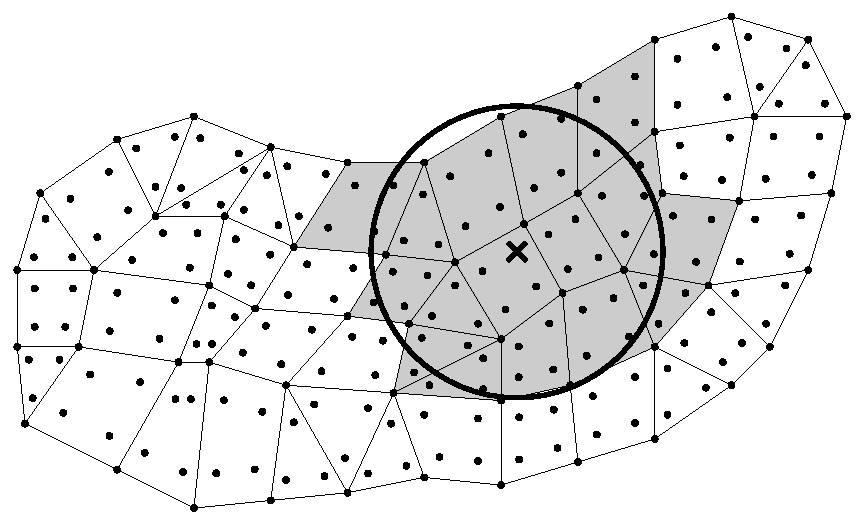
\includegraphics[width=0.7\textwidth]{pics/ApproxSQ.pdf}
    }
    \caption{Квадратурная аппроксимация области нелокальности.}\label{fig:ApproxSQ}
\end{figure}

Ассемблирование остальных слагаемых из уравнения (\ref{eq:ThermalSLAE}) происходит без каких-либо особенностей, поэтому просто выпишем их без подробного разъяснения деталей
\begin{gather}
	\label{eq:HeatTransferMatrix}
	\widehat{\textbf{K}}^{\alpha}_T =
	\sum\limits_{e \in \Gamma_h}
	\sum\limits_{n,m \in I^{e}}
	\sum\limits_{q \in Q^e}
	w_q \alpha N_n^e (\boldsymbol{x}_q) N_m^e (\boldsymbol{x}_q) J_q^e,
	\\
	\label{eq:HeatTransferVector}
	\textbf{T}^{\alpha} =
	\sum\limits_{e \in \Gamma_h}
	\sum\limits_{n \in I^{e}}
	\sum\limits_{q \in Q^e}
	w_q \alpha N_n^e (\boldsymbol{x}_q) T_{\alpha} (\boldsymbol{x}_q) J_q^e
	\\
	\label{eq:InnerFlux}
	\textbf{Q} =
	\sum\limits_{e \in S_h}
	\sum\limits_{n \in I^e}
	\sum\limits_{q \in Q^e}
	w_q q_V (\boldsymbol{x}_q) J_q^e,
	\\
	\label{eq:OuterFlux}
	\textbf{F} =
	\sum\limits_{e \in \Gamma_h}
	\sum\limits_{n \in I^e}
	\sum\limits_{q \in Q^e}
	w_q f (\boldsymbol{x}_q) J_q^e.
\end{gather}
Аналогично запишем ассемблирование остальных слагаемых и для уравнения (\ref{eq:StressSLAE})
\begin{gather}
	\label{eq:InnerPressure}
	\widehat{\textbf{B}} =
	\sum\limits_{e \in S_h}
	\sum\limits_{n \in I^e}
	\sum\limits_{q \in Q^e}
	w_q \boldsymbol{b} (\boldsymbol{x}_q) J_q^e,
	\\
	\label{eq:OuterPressure}
	\widehat{\textbf{P}} = 
	\sum\limits_{e \in \Gamma_h}
	\sum\limits_{n \in I^e}
	\sum\limits_{q \in Q^e}
	w_q \boldsymbol{p} (\boldsymbol{x}_q) J_q^e,
	\\
	\label{eq:LocalThermalExpansion}
	\widehat{\textbf{E}}^L = 
	\sum\limits_{e \in S_h}
	\sum\limits_{n \in I^e}
	\sum\limits_{q \in Q^e}
	w_q \nabla N_n^e (\boldsymbol{x}_q) \widehat{\mathbf{C}} \cdot \cdot \widehat{\boldsymbol{\alpha}} \Delta T (\boldsymbol{x}_q) J_q^e,
\end{gather}
\begin{multline}
	\label{eq:NonLocalThermalExpansion}
	\widehat{\textbf{E}}^{NL} = 
	\sum\limits_{e \in S_h}
	\sum\limits_{n \in I^e}
	\sum\limits_{q \in Q^e}
	w_q \nabla N_n^e (\boldsymbol{x}_q) J_q^e 
	\times \\ \times
	\sum\limits_{e' \in S_h^q}
	\sum\limits_{q' \in Q^{e'}}
	w_{q'} \varphi (\boldsymbol{x}_q, \boldsymbol{x}_{q'}) \widehat{\mathbf{C}} \cdot \cdot \widehat{\boldsymbol{\alpha}} \Delta T (\boldsymbol{x}_{q'}) J_{q'}^{e'},
\end{multline}
отметим, что при ассемблировании $\widehat{\textbf{E}}^{NL}$ была использована методика квадратурной аппроксимации области нелокальности $S'(\boldsymbol{x})$, которая ранее применялась к матрицам нелокальной телопроводности и жёсткости (\ref{eq:ApproxNonloc}).

\section{Вычисление производных величин}\label{sec:NumericalMethods/FluxStressCalculating}

После решения СЛАУ (\ref{eq:ThermalSLAE}) и (\ref{eq:StressSLAE}) на основе полученных сеточных функций температуры $\textbf{T}$ и перемещения $\widehat{\textbf{U}}$ можем найти их производные величины, такие как плотность тепловых потоков $\boldsymbol{q}$ и напряжения $\widehat{\boldsymbol{\sigma}}$ соответственно. Для этого необходимо вычислить градиенты сеточных функций в квадратурных узлах пользуясь формулами (\ref{eq:ApproxTemperatureGradient}) и (\ref{eq:ApproxStrain}). Далее необходимо аппроксимировать интегралы (\ref{eq:BiotFourier}) и (\ref{eq:DuamelNeumann}), для этого снова воспользуемся процедурой квадратурной аппроксимации области нелокальности, после чего получаем формулы для вычисления вектора плотности теплового потока
\begin{gather}
	\label{eq:ApproxFlux}
	\boldsymbol{q}_q = 
	\left(	
	-p_1 \lambda T_m N^e_{m,k} (\boldsymbol{x}_q)
	-p_2 \sum\limits_{e' \in S_h^q} \sum\limits_{q' \in Q^{e'}} w_{q'} \lambda T_{m'} N^e_{m',k} (\boldsymbol{x}_{q'}) J^{e'}_{q'}
	\right) \boldsymbol{e}_k
\end{gather}
и тензора напряжений
\begin{multline}
	\label{eq:ApproxStress}
	\widehat{\boldsymbol{\sigma}}_q =
	\Biggr(
	p_1 C_{ijkl} \left(\varepsilon_{kl} (\boldsymbol{x}_q) - \alpha_{kl} \Delta T_q \right)
	+\\+
	p_2 \sum\limits_{e' \in S_h^q} \sum\limits_{q' \in Q^{e'}} w_{q'} C_{ijkl} \left(\varepsilon_{kl} (\boldsymbol{x}_{q'}) - \alpha_{kl} \Delta T_{q'} \right) J^{e'}_{q'}
	\Biggr) \boldsymbol{e}_k \otimes \boldsymbol{e}_l,
\end{multline}
где $\boldsymbol{q}_q$, $\widehat{\boldsymbol{\sigma}}_q$ и $\Delta T_q$ --- значения вектора плотности теплового потока, тензора напряжений и разницы температур в квадратурном узле $q$ соответственно.

Для дальнейшего анализа полученных решений, переинтерполируем их из квадратурных узлов в регулярные узлы сетки. Для этого при рассмотрении конкретного узла сетки, необходимо определить ближайшие квадратурные узлы каждого из элементов, в состав которых входит этот узел, после чего необходимо вычислить среднюю величину с учётом площадей элементов. Другими словами, вначале для каждого элемента необходимо решить задачу минимизации с поиском нужного индекса $q^e$
\begin{gather*}
	\min_{e \in E^n} \rho(\boldsymbol{x}_n, \boldsymbol{x}_q) \rightarrow q^e,
	\quad
	n \in S_h
\end{gather*}
где $E^n$ --- множество элементов, которым принадлежит узел $n$. После чего необходимо провести процедуру осреднения с весами, где в качестве весовых множителей использовать площади элементов
\begin{gather*}
	|S^n| = \sum\limits_{e \in E^n} |S^e|,
	\quad
	\boldsymbol{q}_n = \sum\limits_{e \in E^n} \dfrac{\boldsymbol{q}_{q^e} |S^e|}{|S^n|},
	\quad
	\widehat{\boldsymbol{\sigma}}_n = \sum\limits_{e \in E^n} \dfrac{\widehat{\boldsymbol{\sigma}}_{q^e} |S^e|}{|S^n|},
\end{gather*}
где $\boldsymbol{q}_n$ и $\widehat{\boldsymbol{\sigma}}_n$ --- значения плотности теплового потока и напряжений в регулярных узлах сетки соответственно.